\begin{center}
    \Huge{\textbf{\underline{Chapter 0: Introduction}}}
\end{center}

\setcounter{section}{0}

\vspace{0.35cm}

\section{Objectives of This Class}  
\begin{prettyBox}{Objectives}{myblue}  
\begin{itemize}  
    \item Understanding static and dynamic web development.  
    \item Implementing interactive web features.  
    \item Exploring the client-server architecture.  
    \item Learning key web technologies: HTML, CSS, JavaScript, PHP, and MySQL.  
\end{itemize}  
\end{prettyBox}  

\vspace{0.35cm}

\section{Clearing Misconception: Internet \(\neq\) Web}  
\begin{prettyBox}{Internet \(\neq\) Web}{myblue}  
Many people mistakenly believe that the Internet and the Web are the same, 
but they are \textbf{two distinct technologies}. The Internet, developed in the \textbf{1960s},
is a global network that connects computers, while the Web, introduced in \textbf{1989},
is a service that operates on top of the Internet. We will explore this
distinction in more detail in the upcoming section.  
\end{prettyBox}  

\vspace{0.35cm}
\subsection{The Internet}


\begin{prettyBox}{Internet}{myblue}  
As previously discussed, the Internet is older than the Web. It was developed
in the 1960s by  3 researchers : Leonard Kleinrock, Vinton Cerf, and Robert Kahn,
with the goal of \textbf{making communication between distant computers possible}.\\[0.15cm]
Their vision was to create a global network that would hold an online library
for sharing and accessing and even updating vast amounts of data,
a concept that later evolved into what we see today with platforms like Wikipedia.\\[0.15cm]
But to reach the Internet as we know it today, many technologies had to be 
developed to solve various challenges. We will list them below.
\end{prettyBox}  

\vspace{0.25cm}

\subsubsection{Modem}  
\begin{prettyBox}{Modem}{myblue}  
A modem is a hardware device that uses telephone lines to enable communication
between distant machines. It operates using two key functions:  

\begin{itemize}  
    \item \textbf{Modulator}: Converts an analog signal into a binary signal.  
    \item \textbf{Demodulator}: Converts a binary signal back into an analog signal.  
\end{itemize}  

The name "modem" comes from the combination of these two functions:
\textbf{MO}dulator and \textbf{DEM}odulator.  
\end{prettyBox}  

\vspace{0.8cm}

\begin{prettyBox}{Note}{red}  
    A legitimate question arises: why did modems rely on telephone lines? 
Why not create a technology to transmit binary signals directly without conversion?\\[0.2cm]
The answer is that cities were already connected by telephone cables.  
Building an entirely new infrastructure for digital communication would have been extremely costly and time-consuming.  
Instead, leveraging the existing telephone network was the most practical and efficient solution.  
\end{prettyBox}  

\vspace{0.75cm}

\subsubsection{Automatic Switching (Switches)}  
\begin{prettyBox}{Switches}{myblue}  
Linking each machine or location directly to all others is impractical.  
We need a technology that can automatically determine the most efficient route 
(shortest path) for communication.This is why switches were invented.\\[0.15cm]
Additionally, switches provide \textbf{resilience}(Fault-tolerant), ensuring that if one 
path fails, an alternative route can be used to maintain communication.  
\end{prettyBox}  

\vspace{0.75cm}

\subsubsection{IP Addresses}  

\begin{prettyBox}{IP}{myblue}  
As the number of machines grew exponentially, using simple labels to identify
them became impractical.A new system was needed to uniquely identify 
each machine while remaining scalable for the future.This led to the
creation of \textbf{IP addresses}.\\[0.15cm]  
The format:  
\begin{center}  
    \boxed{\text{XXX.XXX.XXX.XXX : Port}} where each XXX \(\in\) \([0,255]\)  
\end{center}  
\end{prettyBox}  

\newpage


\begin{prettyBox}{Note}{red}  
\begin{itemize}  
    \item We will discuss \textbf{ports} further in the course.  
    \item Some countries assign \textbf{dynamic IP addresses} to routers,
but internet providers can still track history and identify the original source.  
    \item Over the years, the internet has become a global network,
with undersea cables linking countries.  
\end{itemize}  
\end{prettyBox} 

\vspace{0.35cm}


\subsection{Web}  
\begin{prettyBox}{Web}{myblue}  
    The web emerged much later than the internet. It is a \textbf{service} that leverages the internet,  
similar to how software (the web) operates on hardware (the internet).\\[0.15cm]  
It was created in \textbf{1989} by \textbf{Tim Berners-Lee} to help physicists at \textbf{CERN}  
organize and access their research easily, regardless of their machine's operating system.  
This led to the birth of the first web page, built using \textbf{HTML} and hyperlinks,  
giving rise to the \textbf{World Wide Web (WWW)}.  
\end{prettyBox}  

\vspace{0.5cm}

\begin{prettyBox}{Note}{red}
\begin{itemize}
    \item Tim Berners-Lee created the foundations of the web, including the first web server,  
        \textbf{HTML}, and \textbf{HTTP}.
    \item He has also expressed disappointment that the web did not evolve as
he originally envisioned, as many people now associate it solely with social
media, moving away from its original purpose of sharing and accessing 
information.
\end{itemize}
\end{prettyBox}

\vspace{0.65cm}

\subsubsection{DNS}
\begin{prettyBox}{DNS}{myblue}
To host a website, we use servers that are accessible on the internet 
through a public IP address. The issue is that while IP addresses work
well for machines, most humans cannot easily remember them.\\[0.15cm]  
This is why we needed a way to label websites with \textbf{domain names},
managed by the \textbf{DNS (Domain Name System)}. DNS stores a table that maps 
domain names to their corresponding IP addresses. This allows users to browse
the web using domain names, and then the browser requests the IP address from
the \textbf{DNS}, which redirects the request to the correct server.
\end{prettyBox}

\vspace{0.3cm}

\begin{prettyBox}{Note}{red}
\begin{itemize}
    \item Both the domain name and its corresponding IP address work when  
        accessing a website in the browser.
    \item Some people try to exploit domain names by creating fake websites  
        with similar names to steal user data. However, DNS security has improved,  
        and modern browsers now flag uncertified and unsecure websites.
    \item It is possible to get the public ip of a domain using the \textbf{nslookup} command
\end{itemize}
\end{prettyBox}


\newpage
\null
\textbf{\underline{Nslookup Example}}
\vspace{0.25cm}
\begin{center}
    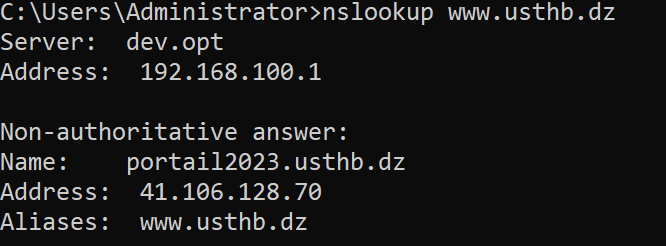
\includegraphics[width=0.6\textwidth]{Chapters/Diagram/Intro/usthbIP.PNG}
\end{center}


\vspace{1.75cm}

\textbf{\underline{DNS Diagram}}
\begin{center}
    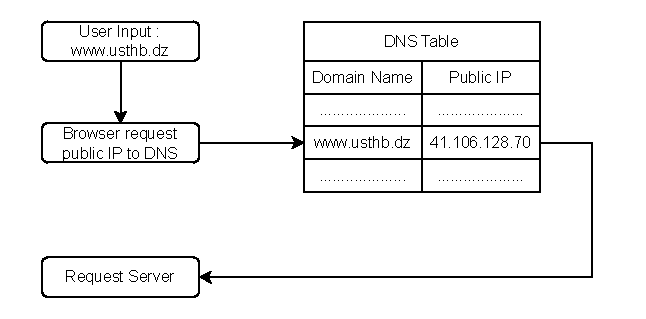
\includegraphics[width=0.7\textwidth]{Chapters/Diagram/Intro/web0.1.drawio.pdf}
\end{center}

\newpage

\subsubsection{Website \& Web Pages}
\begin{prettyBox}{Website \& Web Pages}{myblue}
A website consists of multiple web pages that users can browse through hyperlinks,  
whether they are internal (linking within the same website) or external (linking to a different
website). Each web page has its own \textbf{URL(Uniform Resource Locator)}, and each website has a domain name.
\end{prettyBox}

\vspace{1cm}

\subsubsection{Technologies Involved in Creating a Website}
\begin{prettyBox}{Technologies}{myblue}
\begin{itemize}
    \item \textbf{HTML (HyperText Markup Language):} The backbone and structure of a website.
    \item \textbf{CSS (Cascading Style Sheets):} Used to style fonts, colors, and layouts.
    \item \textbf{JS (JavaScript):} Makes the website interactive.
    \item \textbf{Server-Side Languages:} Various languages can be used, such as PHP, Java, Python, etc.
    \item \textbf{DBMS (Database Management System):} Ensures data persistence, e.g., MySQL, Oracle, etc.
\end{itemize}
\end{prettyBox}

\vspace{1cm}


\subsubsection{Abstraction to the User}
\begin{prettyBox}{Abstraction}{myblue}
There is an abstraction for the user. One might wonder what really happens after entering a 
\textbf{URL}.\\[0.1cm]  
When a URL is entered, an \textbf{HTTP (HyperText Transfer Protocol)} request is sent between the web browser and the web server.
The server responds by sending a copy of the HTML file, which the browser then interprets and 
renders. Users can inspect and even modify the HTML in their browser. However, 
since it is just a local copy, any changes made will not affect the server. If the 
page is refreshed, it will revert to its original state.
\end{prettyBox}

\vspace{0.5cm}

\begin{center}
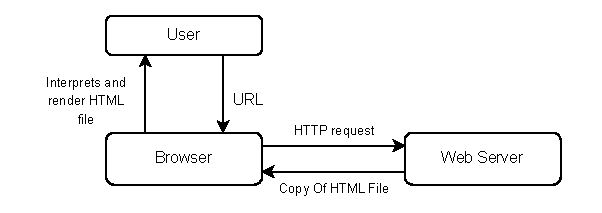
\includegraphics[width=0.7\textwidth]{Chapters/Diagram/Intro/web0.2.drawio.pdf}
\end{center}

\newpage

\subsubsection{Static \& Dynamic Websites}
\begin{prettyBox}{Static \& Dynamic}{myblue}
    The terms \textbf{static} and \textbf{dynamic} refer to how a website's content is updated and displayed:  
\begin{itemize}
    \item \textbf{Static Website}:
        \begin{itemize}
            \item The coder must manually update the content in the code.
            \item No database is used.
            \item The website's content remains the same unless manually updated.
        \end{itemize}
    \item \textbf{Dynamic Website}:
       \begin{itemize}
        \item Content changes dynamically based on user requests.
        \item Uses a database to store and retrieve data.
        \item Requires a server-side language (e.g., PHP, Java, Python).
       \end{itemize}
\end{itemize}
\end{prettyBox}


\vspace{1cm}

\textbf{\underline{Static Website}}
\begin{center}
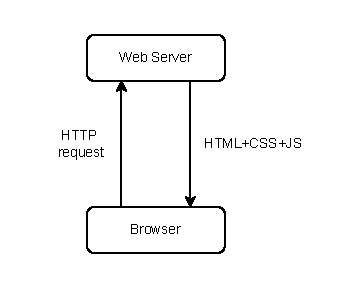
\includegraphics[width=0.5\textwidth]{Chapters/Diagram/Intro/static.drawio.pdf}
\end{center}


\newpage
\textbf{\underline{Dynamic Website}}
\begin{center}
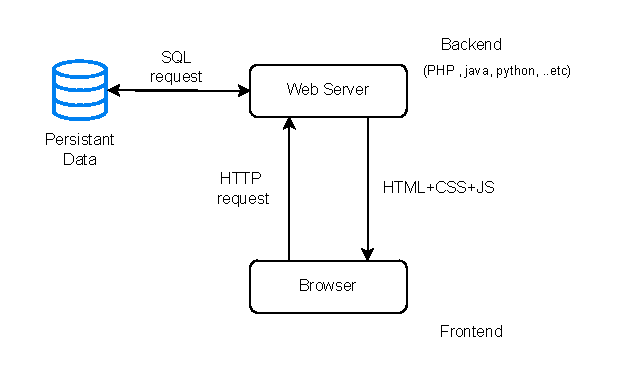
\includegraphics[width=0.7\textwidth]{Chapters/Diagram/Intro/dynamic.drawio.pdf}
\end{center}



